\chapter{Requirements}
\label{chap:requirements}

Requirements identification was critical to the project's success. Primary research was undertaken to understand real user preferences from a list of proposed functionalities. These were used to understand the wants and needs of the artefact. It was critical to declare clear and concise requirements to ensure absolute clarity throughout the project. This chapter discusses all requirements gathering methods used, including the final requirements found as a result of this process.

\section{Requirements Gathering}
\label{requirements:gathering}

Requirements were gathered via multiple channels, initially, research was undertaken to understand the offerings of current solutions to gather a list of potential functionalities. These were then taken to the client to set out a base set of user requirements to be used in primary research. A simple research application was developed to collect the opinions of cyclists in the general public, enabling participants to order a subset of a wider list in order of preference \see{fig:researchapp}.

\section{Identifying Users}
\label{requirements:identifyingusers} 
The aims highlighted the need to expand the route planning functionalities available to cyclists \see{intro:aimsandobjectives}. Multiple user groups were identified from this:
\begin{itemize}
  \item Commuter - A commuter would require a simple round trip route, likely focused on ease of ride and speed taken to commute.
  \item Regular Cyclists - A cyclist who focuses on planning a ride tailored to their skill level. Wants multiple route options with varying levels of intensity.
  \item Pro Cyclists - A pro cyclist would require a deeper level of insight into each planned route, including a range of customisability and integration with fitness applications.
\end{itemize}


\section{Requirements Specification}
\label{requirements:specification}

User stories were established through various methods: regular face-to-face meetings were conducted with the client and research was conducted through a web application built to understand the users' preferred functionality \see{fig:researchapp}. Each user story was broken down into specific system requirements. The requirements have been ranked using the MoSCoW model; this demonstrated each requirement's level of importance consequently reducing the time spent on the less-necessary requirements. The MoSCoW model was the most appropriate choice in prioritising requirements because of the research undertaken with real-world users, utilising the data collected on user preferences \see{fig:userfeedback01}\see{fig:features}.

\begin{figure}[!h]
  \centering
  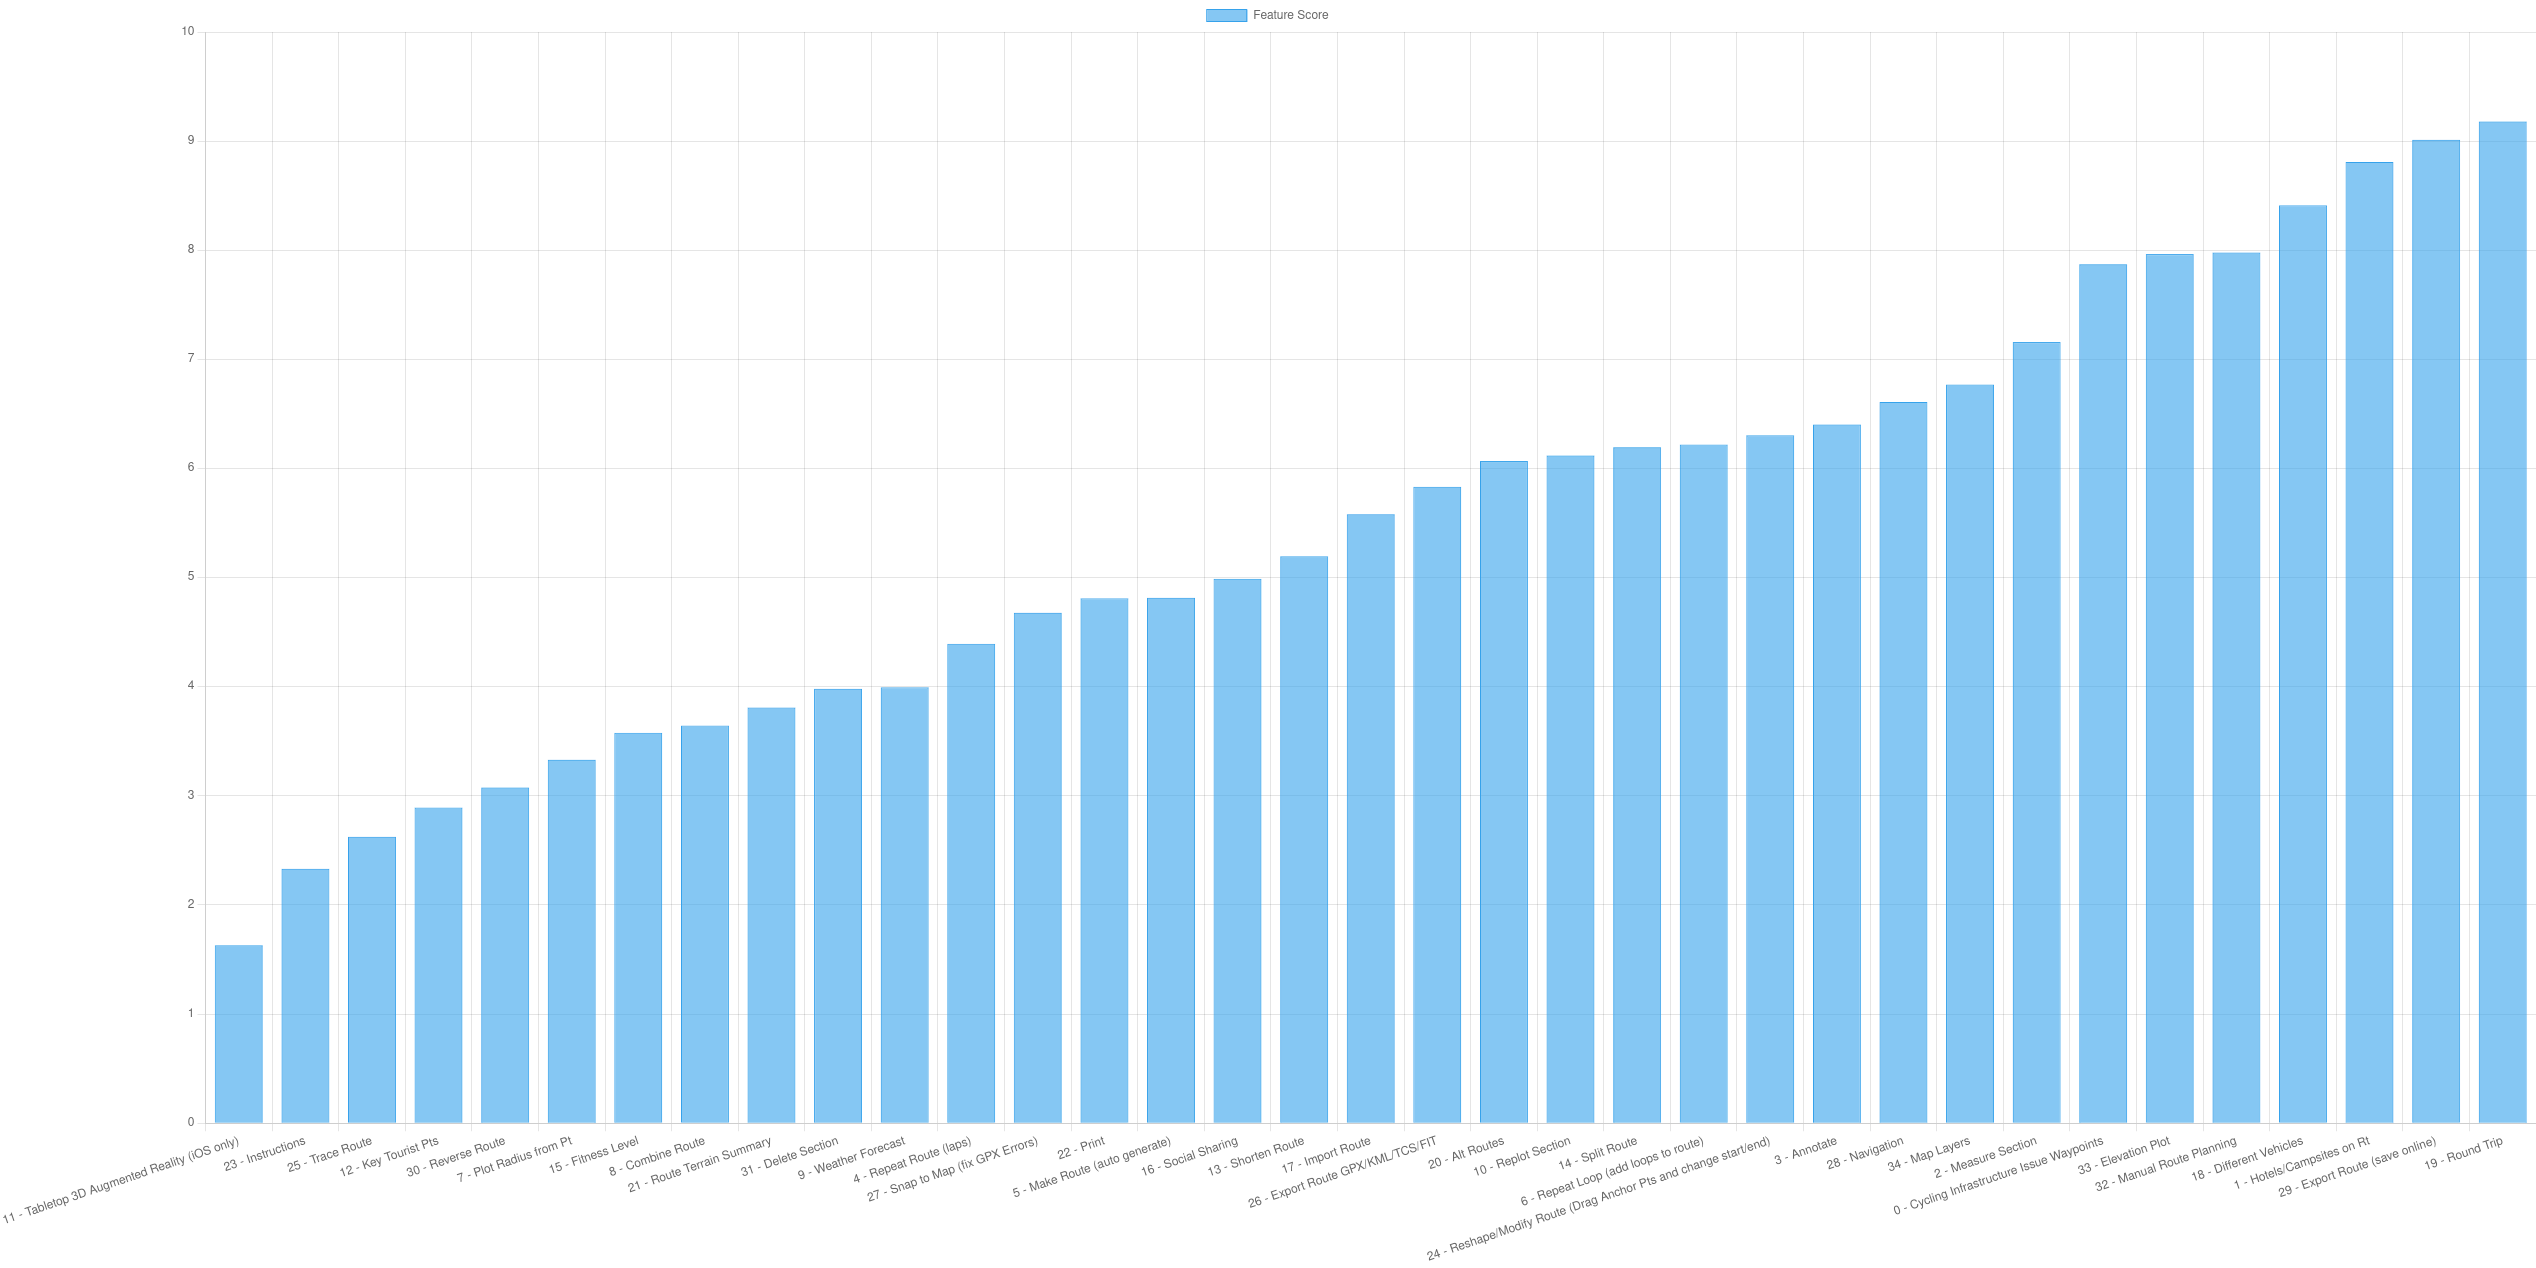
\includegraphics[width=400px]{figures/logarithmic-scoring.png}
  \caption{User Feedback}
  \label{fig:userfeedback01}
\end{figure}

\begin{figure}
  \centering
  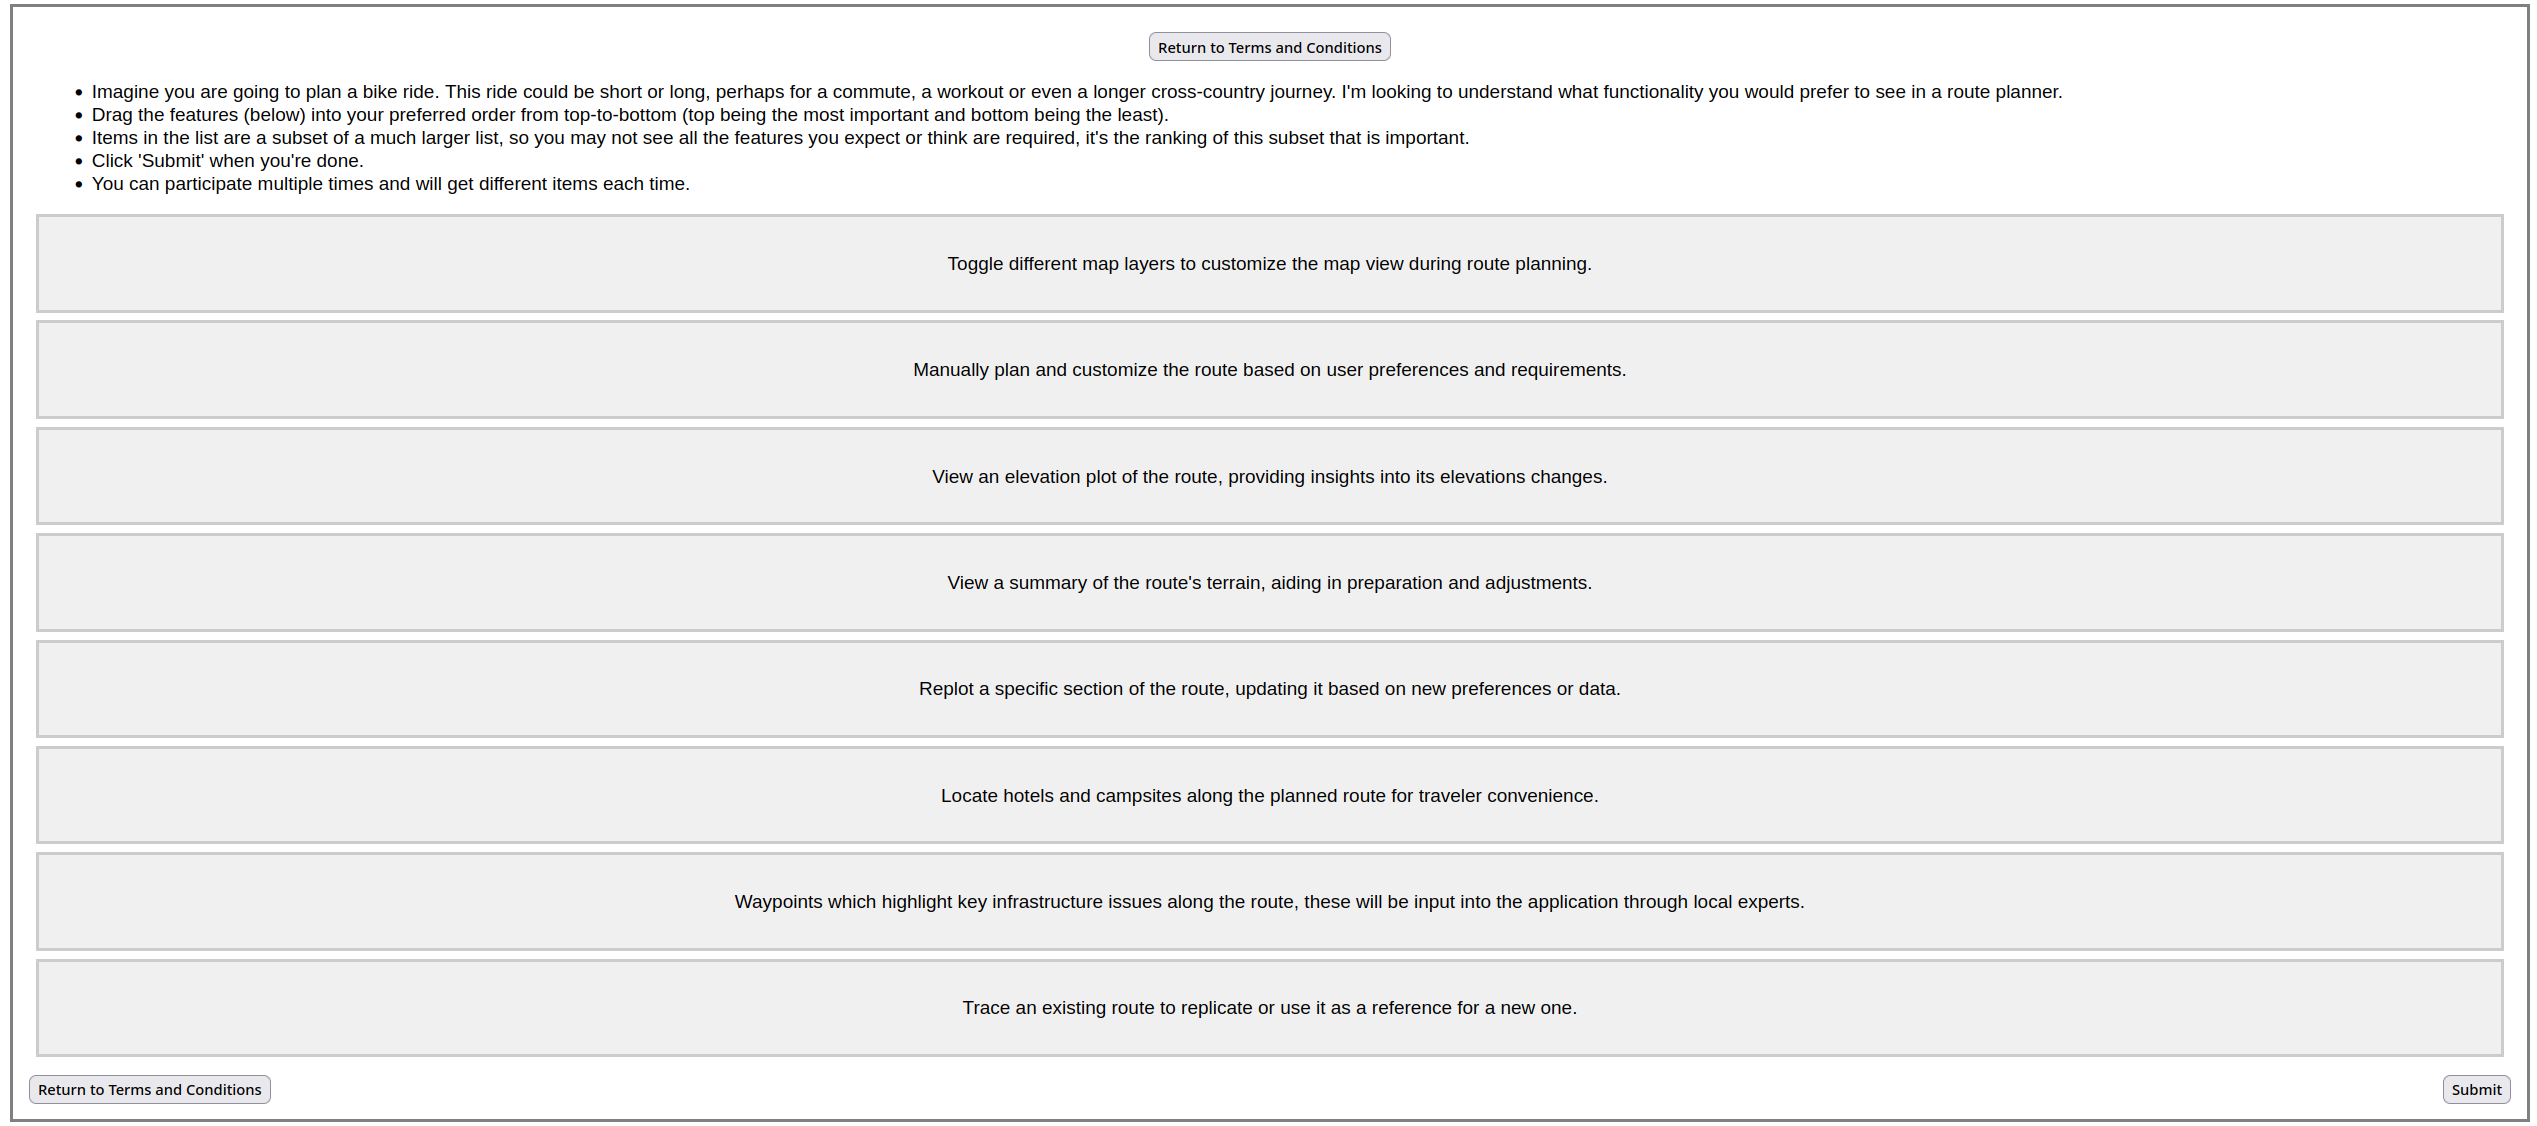
\includegraphics[width=400px]{figures/research-application.png}
  \caption{Firebase Research Application}
  \label{fig:researchapp}
\end{figure}

\clearpage
\section{Elicited Requirements}
\label{requirements:user-stories}

The elicited requirements were the result of discussions with the client and the primary research undertaken \see{requirements:specification}. Each user story was divided into multiple acceptance criteria/system requirements and was segregated into a table per user story.

\begin{table}[!htb]
  \caption{User Story 01}
  \label{tab:user-story-01}
  \begin{tabular}{ m{1cm} m{11cm} m{1cm} }
  \hline
  \multicolumn{3}{p{13cm}}{As a user, I want a page that allows me to configure my starting and destination location to plan a route.}\\ 
  \hline
  ID & Acceptance Criteria / System Requirements & Priority\\
  \hline
  \label{SR:1}SR1 & The system must provide a route configuration panel. & Must \\
  \label{SR:2}SR2 & The route configuration page must provide a starting and destination location input field. & Must\\
  \label{SR:3}SR3 & The route configuration page should suggest accurate geolocations based on the location inputs. & Must\\ 
  \label{SR:4}SR4 & The route configuration page must determine the geolocation based on the user input. & Must\\ 
  \label{SR:5}SR5 & The route configuration page must plan the route once two or more locations are input. & Must\\ 
  \hline
  \end{tabular}
\end{table}

\begin{table}[!htb]
  \caption{User Story 02}
  \label{tab:user-story-02}
  \begin{tabular}{ m{1cm} m{11cm} m{1cm} }
  \hline
  \multicolumn{3}{p{13cm}}{As a user, I want to change preferences to allow me to customise the route, including avoiding certain road types and road altitudes.}\\ 
  \hline
  ID & Acceptance Criteria / System Requirements & Priority\\
  \hline
  \label{SR:6}SR6 & The system must provide an overlay window to allow the user to update routing preferences. & Must \\
  \label{SR:7}SR7 & The update preferences overlay must provide options to 'avoid' along the route. & Must\\
  \label{SR:8}SR8 & The update preferences overlay must provide a 'via' user input field. & Should\\ 
  \label{SR:9}SR9 & The update preferences overlay must provide a 'leave time' user input field. & Should\\ 
  \label{SR:10}SR10 & The update preferences overlay must provide a 'arrive time' user input field. & Should\\ 
  \label{SR:11}SR11 & The update preferences overlay must provide a 'round trip' user input field. & Could\\ 
  \hline
  \end{tabular}
\end{table}

\begin{table}[!htb]
  \caption{User Story 03}
  \label{tab:user-story-03}
  \begin{tabular}{ m{1cm} m{11cm} m{1cm} }
  \hline
  \multicolumn{3}{p{13cm}}{As a user, I want to be able to export the planned route for use on my mobile phone or GPS device.}\\ 
  \hline
  ID & Acceptance Criteria / System Requirements & Priority\\
  \hline
  \label{SR:12}SR12 & The system must provide an option to export the planned route. & Must \\
  \label{SR:13}SR13 & The system must provide an export feature to export the route to the 'GPX' file format. & Must\\
  \label{SR:14}SR14 & The system must provide an export feature to export the route to the 'GeoJSON' file format. & Should\\ 
  \label{SR:15}SR15 & The system must provide an export online (to Google Drive, OneDrive and/or other cloud services) & Must\\
  \hline
  \end{tabular}
\end{table}

\begin{table}[!htb]
  \caption{User Story 04}
  \label{tab:user-story-04}
  \begin{tabular}{ m{1cm} m{11cm} m{1cm} }
  \hline
  \multicolumn{3}{p{13cm}}{As a user, I want to share my route with other people.}\\ 
  \hline
  ID & Acceptance Criteria / System Requirements & Priority\\
  \hline
  \label{SR:16}SR16 & The system must provide a share functionality overlay. & Should \\
  \label{SR:17}SR17 & The share overlay must provide an option to share direct over email. & Should\\
  \label{SR:18}SR18 & The system must provide an option to share the route direct to Strava. & Could\\ 
  \hline
  \end{tabular}
\end{table}

\begin{table}[!htb]
  \caption{User Story 05}
  \label{tab:user-story-05}
  \begin{tabular}{ m{1cm} m{11cm} m{1cm} }
  \hline
  \multicolumn{3}{p{13cm}}{As a user, I want to be provided with route suggestions based on predicted weather conditions over the week.}\\ 
  \hline
  ID & Acceptance Criteria / System Requirements & Priority\\
  \hline
  \label{SR:19}SR19 & The system must provide the user with a weather condition overlay. & Must \\
  \label{SR:20}SR20 & The weather condition overlay must provide the user with the weather for the current day. & Must\\
  \label{SR:21}SR21 & The weather condition overlay must provide the user with the weather for the next week. & Should\\
  \label{SR:22}SR22 & The weather condition overlay must provide the user with the option to enable weather conditions in the route planning algorithm. & Could\\ 
  \label{SR:23}SR23 & The weather condition overlay must provide the user with suggestions on the best days to cycle. & Could\\
  \label{SR:24}SR24 & An option to include weather in route planning should be provided, ensuring the user enters the planned day to ride & Could\\ 
  \hline
  \end{tabular}
\end{table}

\begin{table}[!htb]
  \caption{User Story 06}
  \label{tab:user-story-06}
  \begin{tabular}{ m{1cm} m{11cm} m{1cm} }
  \hline
  \multicolumn{3}{p{13cm}}{As a user, I want to view the route in detail and get information about parts of the route.}\\ 
  \hline
  ID & Acceptance Criteria / System Requirements & Priority\\
  \hline
  \label{SR:25}SR25 & The system must provide the user with an interactive map to display the planned route. & Must \\
  \label{SR:26}SR26 & The interactive map must allow the user to zoom into parts of the planned route. & Must\\
  \label{SR:27}SR27 & The interactive map must allow the user to select parts of the route and receive detailed information about that subsection of the route. & Should\\
  \label{SR:28}SR28 & The interactive map must allow the user to select and drag the planned route to modify its path. & Should\\ 
  \label{SR:29}SR29 & The system must display an elevation graph for the planned route beneath the interactive map. & Should\\
  \label{SR:30}SR30 & The system must allow the user to measure chosen sections of the route & Must\\
  \label{SR:31}SR31 & The system must provide multiple map layers to give users the greater options when viewing the route & Must\\ 
  \hline
  \end{tabular}
\end{table}

\begin{table}[!htb]
  \caption{User Story 07}
  \label{tab:user-story-07}
  \begin{tabular}{ m{1cm} m{11cm} m{1cm} }
  \hline
  \multicolumn{3}{p{13cm}}{As a user, I want the ability to add and utilise hazard/infrastructure waypoints to be considered in route planning.}\\ 
  \hline
  ID & Acceptance Criteria / System Requirements & Priority\\
  \hline
  \label{SR:32}SR32 & The system must provide a user input modal to input Hazard and Infrastructure Data. & Must \\
  \label{SR:33}SR33 & The hazard input modal must provide a Type drop-down menu based on the OSM Hazard Types. & Must\\
  \label{SR:34}SR34 & The hazard input modal must provide a date entry point to specify the date the hazard was seen. & Should\\
  \label{SR:35}SR35 & The hazard input modal must provide a submit button to add the hazard to the hazard index. & Must\\
  \label{SR:36}SR36 & The infrastructure input modal must provide a Type drop-down menu with different types of cycling/road infrastructure & Must\\
  \label{SR:37}SR37 & The infrastructure input modal must provide a date entry point to specify when the bad infrastructure was found & Must\\
  \label{SR:38}SR38 & The infrastructure input modal must provide an input box providing the user with the option to supply more detail & Should\\
  \label{SR:39}SR39 & Both Hazard and Infrastructure data should be displayed on the map, with an option to toggle on/off, and report errors & Should\\
  \hline
  \end{tabular}
\end{table}

\begin{table}[!htb]
  \caption{User Story 08}
  \label{tab:user-story-08}
  \begin{tabular}{ m{1cm} m{11cm} m{1cm} }
  \hline
  \multicolumn{3}{p{13cm}}{As a user, I want to be able to view key waypoints along the journey such as, accommodation and key tourist points.}\\ 
  \hline
  ID & Acceptance Criteria / System Requirements & Priority\\
  \hline
  \label{SR:40}SR40 & The system must provide a map layer to include key waypoints. & Must \\
  \label{SR:41}SR41 & The waypoint layer must provide locations of accommodation along the route. & Must\\
  \label{SR:42}SR42 & The waypoint layer must provide locations of tourist points along the route & Should\\
  \label{SR:43}SR43 & The waypoint layers must be able to be toggled on and off & Must\\
  \label{SR:44}SR44 & Each waypoint must be clickable to provide extra detail on each point & Must\\
  \label{SR:45} SR45 & Each waypoint must have a button to add stop along the route and the route will be re-plotted via the waypoint. & Should\\
  \hline
  \end{tabular}
\end{table}

\begin{table}[!htb]
  \caption{User Story 09}
  \label{tab:user-story-09}
  \begin{tabular}{ m{1cm} m{11cm} m{1cm} }
  \hline
  \multicolumn{3}{p{13cm}}{As a user, I want select what type of cyclist I am, for example road cyclist and commuter cyclist.}\\ 
  \hline
  ID & Acceptance Criteria / System Requirements & Priority\\
  \hline
  \label{SR:46}SR46 & The system must provide an option within the route planning modal to select the rider type. & Must\\
  \label{SR:47}SR47 & The system must provide an option within the route planning modal to select the fitness level of the rider. & Should\\
  \hline
  \end{tabular}
\end{table}

\begin{table}[!htb]
  \caption{User Story 10}
  \label{tab:user-story-10}
  \begin{tabular}{ m{1cm} m{11cm} m{1cm} }
  \hline
  \multicolumn{3}{p{13cm}}{As a user, I want to be able pre-planned routes from other applications.}\\ 
  \hline
  ID & Acceptance Criteria / System Requirements & Priority\\
  \hline
  \label{SR:48}SR48 & The system must provide an import option for GPX files. & Should\\
  \label{SR:49}SR49 & The system must provide an import option for GeoJSON files. & Should\\
  \hline
  \end{tabular}
\end{table}

\begin{table}[!htb]
  \caption{User Story 11}
  \label{tab:user-story-11}
  \begin{tabular}{ m{1cm} m{11cm} m{1cm} }
  \hline
  \multicolumn{3}{p{13cm}}{As a user, I want to be able to share my route to other services and social media.}\\ 
  \hline
  ID & Acceptance Criteria / System Requirements & Priority\\
  \hline
  \label{SR:50}SR50 & The system must provide an export to Garmin Routes. & Should\\
  \label{SR:51}SR51 & The system must provide an option to share to different social media platforms. & Should\\
  \hline
  \end{tabular}
\end{table}